\documentclass[twoside]{book}

% Packages required by doxygen
\usepackage{fixltx2e}
\usepackage{calc}
\usepackage{doxygen}
\usepackage[export]{adjustbox} % also loads graphicx
\usepackage{graphicx}
\usepackage[utf8]{inputenc}
\usepackage{makeidx}
\usepackage{multicol}
\usepackage{multirow}
\PassOptionsToPackage{warn}{textcomp}
\usepackage{textcomp}
\usepackage[nointegrals]{wasysym}
\usepackage[table]{xcolor}

% Font selection
\usepackage[T1]{fontenc}
\usepackage[scaled=.90]{helvet}
\usepackage{courier}
\usepackage{amssymb}
\usepackage{sectsty}
\renewcommand{\familydefault}{\sfdefault}
\allsectionsfont{%
  \fontseries{bc}\selectfont%
  \color{darkgray}%
}
\renewcommand{\DoxyLabelFont}{%
  \fontseries{bc}\selectfont%
  \color{darkgray}%
}
\newcommand{\+}{\discretionary{\mbox{\scriptsize$\hookleftarrow$}}{}{}}

% Page & text layout
\usepackage{geometry}
\geometry{%
  a4paper,%
  top=2.5cm,%
  bottom=2.5cm,%
  left=2.5cm,%
  right=2.5cm%
}
\tolerance=750
\hfuzz=15pt
\hbadness=750
\setlength{\emergencystretch}{15pt}
\setlength{\parindent}{0cm}
\setlength{\parskip}{3ex plus 2ex minus 2ex}
\makeatletter
\renewcommand{\paragraph}{%
  \@startsection{paragraph}{4}{0ex}{-1.0ex}{1.0ex}{%
    \normalfont\normalsize\bfseries\SS@parafont%
  }%
}
\renewcommand{\subparagraph}{%
  \@startsection{subparagraph}{5}{0ex}{-1.0ex}{1.0ex}{%
    \normalfont\normalsize\bfseries\SS@subparafont%
  }%
}
\makeatother

% Headers & footers
\usepackage{fancyhdr}
\pagestyle{fancyplain}
\fancyhead[LE]{\fancyplain{}{\bfseries\thepage}}
\fancyhead[CE]{\fancyplain{}{}}
\fancyhead[RE]{\fancyplain{}{\bfseries\leftmark}}
\fancyhead[LO]{\fancyplain{}{\bfseries\rightmark}}
\fancyhead[CO]{\fancyplain{}{}}
\fancyhead[RO]{\fancyplain{}{\bfseries\thepage}}
\fancyfoot[LE]{\fancyplain{}{}}
\fancyfoot[CE]{\fancyplain{}{}}
\fancyfoot[RE]{\fancyplain{}{\bfseries\scriptsize Generated by Doxygen }}
\fancyfoot[LO]{\fancyplain{}{\bfseries\scriptsize Generated by Doxygen }}
\fancyfoot[CO]{\fancyplain{}{}}
\fancyfoot[RO]{\fancyplain{}{}}
\renewcommand{\footrulewidth}{0.4pt}
\renewcommand{\chaptermark}[1]{%
  \markboth{#1}{}%
}
\renewcommand{\sectionmark}[1]{%
  \markright{\thesection\ #1}%
}

% Indices & bibliography
\usepackage{natbib}
\usepackage[titles]{tocloft}
\setcounter{tocdepth}{3}
\setcounter{secnumdepth}{5}
\makeindex

% Hyperlinks (required, but should be loaded last)
\usepackage{ifpdf}
\ifpdf
  \usepackage[pdftex,pagebackref=true]{hyperref}
\else
  \usepackage[ps2pdf,pagebackref=true]{hyperref}
\fi
\hypersetup{%
  colorlinks=true,%
  linkcolor=blue,%
  citecolor=blue,%
  unicode%
}

% Custom commands
\newcommand{\clearemptydoublepage}{%
  \newpage{\pagestyle{empty}\cleardoublepage}%
}

\usepackage{caption}
\captionsetup{labelsep=space,justification=centering,font={bf},singlelinecheck=off,skip=4pt,position=top}

%===== C O N T E N T S =====

\begin{document}

% Titlepage & ToC
\hypersetup{pageanchor=false,
             bookmarksnumbered=true,
             pdfencoding=unicode
            }
\pagenumbering{roman}
\begin{titlepage}
\vspace*{7cm}
\begin{center}%
{\Large My Project }\\
\vspace*{1cm}
{\large Generated by Doxygen 1.8.11}\\
\end{center}
\end{titlepage}
\clearemptydoublepage
\tableofcontents
\clearemptydoublepage
\pagenumbering{arabic}
\hypersetup{pageanchor=true}

%--- Begin generated contents ---
\chapter{Class Index}
\section{Class List}
Here are the classes, structs, unions and interfaces with brief descriptions\+:\begin{DoxyCompactList}
\item\contentsline{section}{\hyperlink{class_casual}{Casual} }{\pageref{class_casual}}{}
\item\contentsline{section}{\hyperlink{class_faculty}{Faculty} }{\pageref{class_faculty}}{}
\item\contentsline{section}{\hyperlink{class_officer}{Officer} }{\pageref{class_officer}}{}
\item\contentsline{section}{\hyperlink{class_permanent}{Permanent} }{\pageref{class_permanent}}{}
\item\contentsline{section}{\hyperlink{class_staff}{Staff} }{\pageref{class_staff}}{}
\item\contentsline{section}{\hyperlink{class_typist}{Typist} }{\pageref{class_typist}}{}
\end{DoxyCompactList}

\chapter{File Index}
\section{File List}
Here is a list of all files with brief descriptions\+:\begin{DoxyCompactList}
\item\contentsline{section}{\hyperlink{person_8cpp}{person.\+cpp} }{\pageref{person_8cpp}}{}
\end{DoxyCompactList}

\chapter{Class Documentation}
\hypertarget{structdate}{}\section{date Struct Reference}
\label{structdate}\index{date@{date}}
\subsection*{Public Attributes}
\begin{DoxyCompactItemize}
\item 
int \hyperlink{structdate_a76f88239963cde7603622f6527e55a08}{dd}
\item 
int \hyperlink{structdate_ad63f86912f69ef43c342a0d4328431f0}{mm}
\item 
int \hyperlink{structdate_a2abeb95ba2a1a5cdcf1cd3667d9ea3ca}{yyyy}
\end{DoxyCompactItemize}


\subsection{Member Data Documentation}
\index{date@{date}!dd@{dd}}
\index{dd@{dd}!date@{date}}
\subsubsection[{\texorpdfstring{dd}{dd}}]{\setlength{\rightskip}{0pt plus 5cm}int date\+::dd}\hypertarget{structdate_a76f88239963cde7603622f6527e55a08}{}\label{structdate_a76f88239963cde7603622f6527e55a08}
\index{date@{date}!mm@{mm}}
\index{mm@{mm}!date@{date}}
\subsubsection[{\texorpdfstring{mm}{mm}}]{\setlength{\rightskip}{0pt plus 5cm}int date\+::mm}\hypertarget{structdate_ad63f86912f69ef43c342a0d4328431f0}{}\label{structdate_ad63f86912f69ef43c342a0d4328431f0}
\index{date@{date}!yyyy@{yyyy}}
\index{yyyy@{yyyy}!date@{date}}
\subsubsection[{\texorpdfstring{yyyy}{yyyy}}]{\setlength{\rightskip}{0pt plus 5cm}int date\+::yyyy}\hypertarget{structdate_a2abeb95ba2a1a5cdcf1cd3667d9ea3ca}{}\label{structdate_a2abeb95ba2a1a5cdcf1cd3667d9ea3ca}


The documentation for this struct was generated from the following file\+:\begin{DoxyCompactItemize}
\item 
\hyperlink{person_8cpp}{person.\+cpp}\end{DoxyCompactItemize}

\hypertarget{class_person}{}\section{Person Class Reference}
\label{class_person}\index{Person@{Person}}
\subsection*{Public Member Functions}
\begin{DoxyCompactItemize}
\item 
void \hyperlink{class_person_abfb9b11cae76f0907077ee1865adf375}{input} ()
\item 
void \hyperlink{class_person_a1ff5816f026c35843137266fc90a8002}{display} ()
\end{DoxyCompactItemize}
\subsection*{Friends}
\begin{DoxyCompactItemize}
\item 
ofstream \& \hyperlink{class_person_a327a74c40e134e4da13cc5b16cf5c24b}{operator$<$$<$} (ofstream \&, const \hyperlink{class_person}{Person} $\ast$)
\item 
ifstream \& \hyperlink{class_person_aafbce4bf346d34deff9c806efc01a49f}{operator$>$$>$} (ifstream \&, \hyperlink{class_person}{Person} $\ast$)
\end{DoxyCompactItemize}


\subsection{Member Function Documentation}
\index{Person@{Person}!display@{display}}
\index{display@{display}!Person@{Person}}
\subsubsection[{\texorpdfstring{display()}{display()}}]{\setlength{\rightskip}{0pt plus 5cm}void Person\+::display (
\begin{DoxyParamCaption}
{}
\end{DoxyParamCaption}
)}\hypertarget{class_person_a1ff5816f026c35843137266fc90a8002}{}\label{class_person_a1ff5816f026c35843137266fc90a8002}
\index{Person@{Person}!input@{input}}
\index{input@{input}!Person@{Person}}
\subsubsection[{\texorpdfstring{input()}{input()}}]{\setlength{\rightskip}{0pt plus 5cm}void Person\+::input (
\begin{DoxyParamCaption}
{}
\end{DoxyParamCaption}
)}\hypertarget{class_person_abfb9b11cae76f0907077ee1865adf375}{}\label{class_person_abfb9b11cae76f0907077ee1865adf375}


\subsection{Friends And Related Function Documentation}
\index{Person@{Person}!operator$<$$<$@{operator$<$$<$}}
\index{operator$<$$<$@{operator$<$$<$}!Person@{Person}}
\subsubsection[{\texorpdfstring{operator$<$$<$}{operator<<}}]{\setlength{\rightskip}{0pt plus 5cm}ofstream\& operator$<$$<$ (
\begin{DoxyParamCaption}
\item[{ofstream \&}]{out, }
\item[{const {\bf Person} $\ast$}]{p}
\end{DoxyParamCaption}
)\hspace{0.3cm}{\ttfamily [friend]}}\hypertarget{class_person_a327a74c40e134e4da13cc5b16cf5c24b}{}\label{class_person_a327a74c40e134e4da13cc5b16cf5c24b}
\index{Person@{Person}!operator$>$$>$@{operator$>$$>$}}
\index{operator$>$$>$@{operator$>$$>$}!Person@{Person}}
\subsubsection[{\texorpdfstring{operator$>$$>$}{operator>>}}]{\setlength{\rightskip}{0pt plus 5cm}ifstream\& operator$>$$>$ (
\begin{DoxyParamCaption}
\item[{ifstream \&}]{in, }
\item[{{\bf Person} $\ast$}]{p}
\end{DoxyParamCaption}
)\hspace{0.3cm}{\ttfamily [friend]}}\hypertarget{class_person_aafbce4bf346d34deff9c806efc01a49f}{}\label{class_person_aafbce4bf346d34deff9c806efc01a49f}


The documentation for this class was generated from the following file\+:\begin{DoxyCompactItemize}
\item 
\hyperlink{person_8cpp}{person.\+cpp}\end{DoxyCompactItemize}

\chapter{File Documentation}
\hypertarget{person_8cpp}{}\section{person.\+cpp File Reference}
\label{person_8cpp}\index{person.\+cpp@{person.\+cpp}}
{\ttfamily \#include $<$iostream$>$}\\*
{\ttfamily \#include $<$stdlib.\+h$>$}\\*
{\ttfamily \#include $<$fstream$>$}\\*
Include dependency graph for person.\+cpp\+:
\nopagebreak
\begin{figure}[H]
\begin{center}
\leavevmode
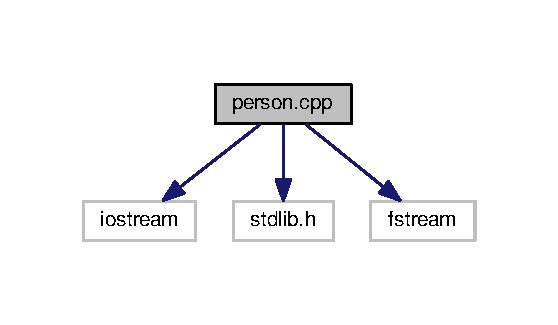
\includegraphics[width=268pt]{person_8cpp__incl}
\end{center}
\end{figure}
\subsection*{Classes}
\begin{DoxyCompactItemize}
\item 
struct \hyperlink{structdate}{date}
\item 
class \hyperlink{class_person}{Person}
\end{DoxyCompactItemize}
\subsection*{Typedefs}
\begin{DoxyCompactItemize}
\item 
typedef struct \hyperlink{structdate}{date} \hyperlink{person_8cpp_ab8e06a427a2b4ef4f4d0cb455c5af012}{Date}
\end{DoxyCompactItemize}
\subsection*{Functions}
\begin{DoxyCompactItemize}
\item 
ofstream \& \hyperlink{person_8cpp_a01861370261121fdc63ea10f5a844364}{operator$<$$<$} (ofstream \&out, const \hyperlink{person_8cpp_ab8e06a427a2b4ef4f4d0cb455c5af012}{Date} \&dob)
\item 
ifstream \& \hyperlink{person_8cpp_a13869537a181034c7922c49af76329e3}{operator$>$$>$} (ifstream \&in, \hyperlink{person_8cpp_ab8e06a427a2b4ef4f4d0cb455c5af012}{Date} \&dob)
\item 
ofstream \& \hyperlink{person_8cpp_a7075ab6fbe9e271c40f328923c73b408}{operator$<$$<$} (ofstream \&out, const \hyperlink{class_person}{Person} $\ast$p)
\item 
ifstream \& \hyperlink{person_8cpp_afb2a177ce772936d2a1b130c2cfd164f}{operator$>$$>$} (ifstream \&in, \hyperlink{class_person}{Person} $\ast$p)
\item 
int \hyperlink{person_8cpp_ae66f6b31b5ad750f1fe042a706a4e3d4}{main} ()
\end{DoxyCompactItemize}


\subsection{Typedef Documentation}
\index{person.\+cpp@{person.\+cpp}!Date@{Date}}
\index{Date@{Date}!person.\+cpp@{person.\+cpp}}
\subsubsection[{\texorpdfstring{Date}{Date}}]{\setlength{\rightskip}{0pt plus 5cm}typedef struct {\bf date}  {\bf Date}}\hypertarget{person_8cpp_ab8e06a427a2b4ef4f4d0cb455c5af012}{}\label{person_8cpp_ab8e06a427a2b4ef4f4d0cb455c5af012}


\subsection{Function Documentation}
\index{person.\+cpp@{person.\+cpp}!main@{main}}
\index{main@{main}!person.\+cpp@{person.\+cpp}}
\subsubsection[{\texorpdfstring{main()}{main()}}]{\setlength{\rightskip}{0pt plus 5cm}int main (
\begin{DoxyParamCaption}
{}
\end{DoxyParamCaption}
)}\hypertarget{person_8cpp_ae66f6b31b5ad750f1fe042a706a4e3d4}{}\label{person_8cpp_ae66f6b31b5ad750f1fe042a706a4e3d4}
\index{person.\+cpp@{person.\+cpp}!operator$<$$<$@{operator$<$$<$}}
\index{operator$<$$<$@{operator$<$$<$}!person.\+cpp@{person.\+cpp}}
\subsubsection[{\texorpdfstring{operator$<$$<$(ofstream \&out, const Date \&dob)}{operator<<(ofstream &out, const Date &dob)}}]{\setlength{\rightskip}{0pt plus 5cm}ofstream\& operator$<$$<$ (
\begin{DoxyParamCaption}
\item[{ofstream \&}]{out, }
\item[{const {\bf Date} \&}]{dob}
\end{DoxyParamCaption}
)}\hypertarget{person_8cpp_a01861370261121fdc63ea10f5a844364}{}\label{person_8cpp_a01861370261121fdc63ea10f5a844364}
\index{person.\+cpp@{person.\+cpp}!operator$<$$<$@{operator$<$$<$}}
\index{operator$<$$<$@{operator$<$$<$}!person.\+cpp@{person.\+cpp}}
\subsubsection[{\texorpdfstring{operator$<$$<$(ofstream \&out, const Person $\ast$p)}{operator<<(ofstream &out, const Person *p)}}]{\setlength{\rightskip}{0pt plus 5cm}ofstream\& operator$<$$<$ (
\begin{DoxyParamCaption}
\item[{ofstream \&}]{out, }
\item[{const {\bf Person} $\ast$}]{p}
\end{DoxyParamCaption}
)}\hypertarget{person_8cpp_a7075ab6fbe9e271c40f328923c73b408}{}\label{person_8cpp_a7075ab6fbe9e271c40f328923c73b408}
\index{person.\+cpp@{person.\+cpp}!operator$>$$>$@{operator$>$$>$}}
\index{operator$>$$>$@{operator$>$$>$}!person.\+cpp@{person.\+cpp}}
\subsubsection[{\texorpdfstring{operator$>$$>$(ifstream \&in, Date \&dob)}{operator>>(ifstream &in, Date &dob)}}]{\setlength{\rightskip}{0pt plus 5cm}ifstream\& operator$>$$>$ (
\begin{DoxyParamCaption}
\item[{ifstream \&}]{in, }
\item[{{\bf Date} \&}]{dob}
\end{DoxyParamCaption}
)}\hypertarget{person_8cpp_a13869537a181034c7922c49af76329e3}{}\label{person_8cpp_a13869537a181034c7922c49af76329e3}
\index{person.\+cpp@{person.\+cpp}!operator$>$$>$@{operator$>$$>$}}
\index{operator$>$$>$@{operator$>$$>$}!person.\+cpp@{person.\+cpp}}
\subsubsection[{\texorpdfstring{operator$>$$>$(ifstream \&in, Person $\ast$p)}{operator>>(ifstream &in, Person *p)}}]{\setlength{\rightskip}{0pt plus 5cm}ifstream\& operator$>$$>$ (
\begin{DoxyParamCaption}
\item[{ifstream \&}]{in, }
\item[{{\bf Person} $\ast$}]{p}
\end{DoxyParamCaption}
)}\hypertarget{person_8cpp_afb2a177ce772936d2a1b130c2cfd164f}{}\label{person_8cpp_afb2a177ce772936d2a1b130c2cfd164f}

%--- End generated contents ---

% Index
\backmatter
\newpage
\phantomsection
\clearemptydoublepage
\addcontentsline{toc}{chapter}{Index}
\printindex

\end{document}
